\documentclass[conference]{IEEEtran}
\usepackage{graphicx}
\usepackage{booktabs}
\usepackage{tikz}
\usetikzlibrary{arrows.meta,positioning,fit}
\usepackage{url}
\usepackage[hidelinks]{hyperref}

\title{StateScout: Defeasible and Reversible Semantic State Abstraction for Web UI Exploration}
\author{\IEEEauthorblockN{Anonymous Author(s)}
\IEEEauthorblockA{Double-anonymous submission}}

\begin{document}
\maketitle

\begin{abstract}
Modern web applications expose many interaction states without changing URL, while timestamps, generated identifiers, and other dynamic content can make equivalent observations appear different. Automated web explorers therefore depend on state abstraction that avoids both false splits, which waste exploration effort, and false merges, which can hide reachable behavior. Prior work has proposed DOM comparators, adaptive abstraction refinement, page fragmentation, neural embeddings, and learned classifiers. This paper studies a complementary question: how should an abstraction assumption be governed after evidence suggests that it is valid?

We present StateScout, an experimental Playwright-based web UI explorer that treats learned state abstraction as an explicit cross-run trust hypothesis. StateScout freezes state identity within each run, quarantines candidate volatility, promotes rules only between runs after scoped repeated observations and stable safe-probe behavior, and tracks rule provenance, freshness, challenge, revocation, cooldown, and restoration. A bounded scheduler prioritizes rule revalidation, while an immutable raw archive preserves historical observations beneath the current projection.

Across a frozen 16-pair controlled corpus, URL-only identity classified 5/16 pairs correctly while the frozen semantic baseline classified 14/16; removing semantic control state reduced correctness to 9/16. Scoped learned volatility resolved a held-out ambiguity benchmark at 6/6. In a controlled drift benchmark, stale abstraction reduced meaningful-state coverage to 0.5 and revocation restored full coverage. The same immutable six-observation archive projected to 3, then 6, then 3 states as trust changed. A five-target public study produced three evaluable targets and zero StateScout run-level errors, while a later replication demonstrated temporal graph variability. Finally, interrupted synthetic and Playwright explorations resumed to the same controlled final graphs as uninterrupted runs.

These results do not establish a universally optimal state classifier. They support a narrower design principle: state abstraction in a web explorer can benefit from explicit cross-run trust management, delayed promotion, defeasible rules, and preservation of historical evidence.
\end{abstract}

\section{Introduction}
Modern web applications are not collections of static pages. A single route can expose dialogs, menus, tabs, asynchronous results, form states, and other interaction states without changing URL. Automated testing systems therefore require a notion of application state richer than navigation history.

This problem has extensive prior art. GUI ripping and event-flow models established automated extraction of interaction models~\cite{memon2003guiripping,memon2007eventflow}. Crawljax showed that AJAX applications can be explored through dynamically inferred state-flow graphs~\cite{mesbah2008crawling,mesbah2012crawljax}. Subsequent work addressed dynamic noise, model inference, feedback-guided exploration, page fragmentation, learned embeddings, and learned state classifiers~\cite{roest2010regression,fard2013feedback,yandrapally2023fraggen,kanaththage2026webembed,liu2026judge}.

The abstraction error is asymmetric. A \emph{false split} represents one meaningful state as several states, inflating the graph and wasting exploration. A \emph{false merge} collapses meaningfully different states. For exploration, false merges are especially dangerous because the system may mark an area as already explored and suppress descendants reachable only from the collapsed distinction.

Most abstraction techniques focus primarily on the current equivalence decision. Figure~\ref{fig:lifecycle} summarizes StateScout's alternative framing. StateScout asks a different question: \emph{what lifecycle should govern an abstraction assumption after evidence suggests that it is valid?}

APE already demonstrates online GUI abstraction refinement/coarsening and model rebuilding from recorded GUI histories~\cite{gu2019ape}. StateScout therefore does not claim novelty for changing an abstraction or rebuilding a model by itself. Its candidate contribution is an explicit \emph{cross-run rule-trust lifecycle}: identity is frozen within a run; candidate rules are quarantined; promotion happens only between runs after scoped and behavioral evidence; later evidence can challenge, revoke, cool down, or restore trust; maintenance can be scheduled under a budget; and preserved raw evidence remains available as trust changes.

We make four contributions:
\begin{enumerate}
  \item \textbf{Run-frozen evidence-backed abstraction.} Candidate volatility is scoped to a protected semantic anchor and cannot mutate the identity function of the run that observes it.
  \item \textbf{Defeasible cross-run rule trust.} Rules have explicit provenance, freshness, challenge, revocation, cooldown/restoration, and bounded selective revalidation.
  \item \textbf{Preserved historical evidence.} Raw semantic observations and transitions remain immutable beneath the active projection, so later trust changes can reinterpret recorded distinctions without rewriting evidence.
  \item \textbf{A frozen reproducible evaluation artifact.} The artifact includes controlled counterexamples and ablations, lifecycle/drift experiments, a public-site repeated-run study with temporal replication, same-origin safe exploration, and checkpoint/resume.
\end{enumerate}



\begin{figure*}[t]
\centering
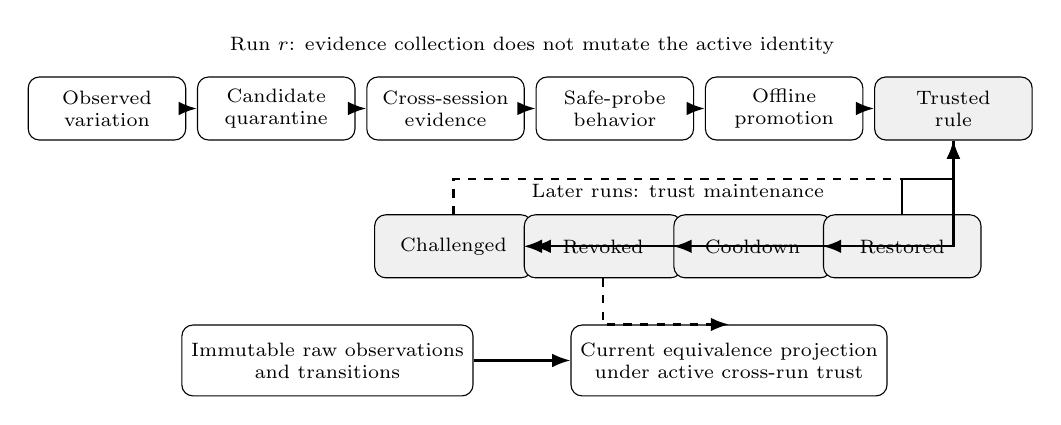
\begin{tikzpicture}[
  >=Latex,
  box/.style={draw, rounded corners, align=center, minimum width=20mm, minimum height=8mm, font=\scriptsize},
  trust/.style={box, fill=gray!12},
  raw/.style={draw, rounded corners, align=center, minimum width=36mm, minimum height=9mm, font=\scriptsize},
  arrow/.style={->, thick}
]
\node[font=\scriptsize] at (5.4,0.8) {Run $r$: evidence collection does not mutate the active identity};

\node[box] (obs) at (0,0) {Observed\\variation};
\node[box] (cand) at (2.15,0) {Candidate\\quarantine};
\node[box] (cross) at (4.30,0) {Cross-session\\evidence};
\node[box] (beh) at (6.45,0) {Safe-probe\\behavior};
\node[box] (prom) at (8.60,0) {Offline\\promotion};
\node[trust] (trusted) at (10.75,0) {Trusted\\rule};

\draw[arrow] (obs) -- (cand);
\draw[arrow] (cand) -- (cross);
\draw[arrow] (cross) -- (beh);
\draw[arrow] (beh) -- (prom);
\draw[arrow] (prom) -- (trusted);

\node[font=\scriptsize] at (7.25,-1.05) {Later runs: trust maintenance};
\node[trust] (chall) at (4.4,-1.75) {Challenged};
\node[trust] (rev) at (6.3,-1.75) {Revoked};
\node[trust] (cool) at (8.2,-1.75) {Cooldown};
\node[trust] (rest) at (10.1,-1.75) {Restored};

\draw[arrow] (trusted.south) |- (chall.east);
\draw[arrow] (chall) -- (rev);
\draw[arrow] (rev) -- (cool);
\draw[arrow] (cool) -- (rest);
\draw[arrow] (rest.north) -- ++(0,0.45) -| (trusted.south);
\draw[arrow, dashed] (chall.north) -- ++(0,0.45) -| (trusted.south);

\node[raw] (archive) at (2.8,-3.2) {Immutable raw observations\\and transitions};
\node[raw] (projection) at (7.9,-3.2) {Current equivalence projection\\under active cross-run trust};
\draw[arrow] (archive) -- (projection);
\draw[arrow, dashed] (rev.south) |- (projection.north);

\end{tikzpicture}
\caption{StateScout treats abstraction as an explicit cross-run trust lifecycle rather than a one-shot equality decision. Promotion occurs only between runs; later evidence can challenge, revoke, or restore trust while raw history remains preserved.}
\label{fig:lifecycle}
\end{figure*}

\section{Background and Related Work}
\subsection{GUI and Web State Models}
GUI ripping and event-flow modeling establish automatic extraction of GUI interaction structure~\cite{memon2003guiripping,memon2007eventflow}. Crawljax extends the idea to client-side web applications and demonstrates why URL identity is inadequate for modern web state~\cite{mesbah2008crawling,mesbah2012crawljax}.

\subsection{Exploration and State Abstraction}
ARTEMIS, WebMate, FEEDEx, AutoBlackTest, and TESTAR-related work span automated exploration, feedback-guided action selection, replay, and inferred GUI models~\cite{artzi2011framework,dallmeier2012webmate,fard2013feedback,mariani2014autoblacktest,mulders2022statemodel,pastorricos2023distributed}. Roest et al. show that comparator pipelines can strip known AJAX dynamism before comparison~\cite{roest2010regression}.

Near-duplicate detection and abstraction have become increasingly sophisticated. MinHash-based structural similarity, fragment-based analysis, neural embeddings, and learned classifiers all provide established approaches to page equivalence~\cite{benbassat2019minhash,yandrapally2023fraggen,kanaththage2026webembed,liu2026judge}. A recent empirical study further shows that exploration strategy and state abstraction interact~\cite{liu2026understanding}.

\subsection{Adaptive Abstraction Refinement}
APE dynamically refines and coarsens an Android GUI abstraction using runtime evidence and rebuilds the model from recorded GUI trees and transitions~\cite{gu2019ape}. Accordingly, StateScout's distinction is not abstraction refinement or model rebuilding in isolation. StateScout freezes the active identity function during each run and changes later abstraction trust through an explicit cross-run object with delayed promotion, freshness, challenge/revocation/restoration, and selective revalidation.

\subsection{Semantic Browser Observations}
Modern browser-agent environments such as WebArena, WorkArena, and BrowserGym expose rich browser representations and accessibility-oriented observations~\cite{zhou2024webarena,drouin2024workarena,chezelles2024browsergym}. StateScout's role/name-oriented semantic controls are therefore an engineering choice rather than a novelty claim.

\section{StateScout}
\subsection{Semantic Observation and Graph}
A semantic observation contains origin/path/query information, title, visible headings, landmarks, accessible dialogs, and semantic controls with selected control state. A state identity function maps an observation to a canonical representation and hash.

Exploration produces a directed graph $G=(V,E)$. The breadth-first frontier stores \texttt{(source state, interaction, replay path)} work and maintains a distinct seen set over \texttt{(source state, interaction)}. Paths may converge and cycles are normal.

\subsection{Replay and Safety}
Because browser execution is sequential, a pending BFS state may no longer be active. StateScout restores its source by returning to the start state, replaying the recorded path, and checking expected intermediate fingerprints before executing the pending action.

Interactions receive deterministic risk classification. The default policy executes only safe interactions, while mutating/destructive actions remain blocked. Navigation is also constrained to a same-origin boundary.

\subsection{From Candidate to Trusted Rule}
StateScout separates observation from trust activation. A varying title/query field first becomes a candidate only when repeated observations share the same protected semantic anchor. The frozen candidate policy requires at least four observations, two sessions, three distinct values, and four behavior-evidence records.

Behavior evidence records bounded safe-probe outcomes. Stable downstream behavior can make a candidate eligible; divergent behavior leaves it quarantined. Promotion occurs offline and affects only a future run.

\subsection{Cross-Run Trust Lifecycle}
Trusted rules carry provenance and freshness. Later rule-scoped evidence can retain, challenge, revoke, or restore trust. The frozen lifecycle uses a 30-day maximum trust age, 7-day maximum evidence age, two conflicting windows to revoke, and two stable windows to restore.

When multiple rules require maintenance, StateScout ranks them under a fixed verification budget using a transparent score combining state urgency, freshness risk, conflict history, and estimated coverage impact. The weights are experimental choices, not claimed optimal.

\subsection{Preserved History and Reprojection}
StateScout keeps raw semantic observations and transitions separate from the current abstraction projection. A trusted rule may alias several raw observations into one projected state. Revocation can expose already-recorded distinctions again. This does not recover interactions that were never explored due to a previous false merge.

\subsection{Checkpoint and Resume}
A logical checkpoint stores the graph, pending BFS queue, complete seen-work set, root replay path, transition-attempt count, evidence errors, and start URL. The payload is SHA-256 protected. StateScout does not snapshot Chromium memory; pending sources are reconstructed through replay.

\section{Methodology}
\subsection{Research Questions}
Table~\ref{tab:rqmap} maps each question to its frozen evidence. \textbf{RQ1---Identity:} How do URL-only and progressively richer semantic identities trade false merges and false splits?

\textbf{RQ2---Contextual abstraction:} Can scoped repeated evidence distinguish measured volatile presentation differences from meaningful state differences?

\textbf{RQ3---Defeasibility:} Can stale trusted abstraction be challenged/revoked, and can recorded distinctions be recovered without mutating raw evidence?

\textbf{RQ4---Bounded maintenance:} Can multiple learned rules be prioritized for revalidation under a fixed budget?

\textbf{RQ5---Operational robustness:} Can safe bounded exploration operate on public targets and resume interrupted controlled exploration without changing the final graph?



\begin{table*}[t]
\caption{Research questions and the frozen evidence used to answer them.}
\label{tab:rqmap}
\centering
\small
\begin{tabular}{p{0.055\textwidth}p{0.30\textwidth}p{0.56\textwidth}}
\toprule
RQ & Question & Frozen evidence \\
\midrule
RQ1 & Identity accuracy & 16 labeled browser-observed pairs; URL-only, v1--v4, and three v4 ablations plus targeted-content diagnostic. \\
RQ2 & Contextual abstraction & Six held-out pairs testing whether anchor-scoped evidence can separate measured volatility from meaningful time/reference values. \\
RQ3 & Defeasibility & Behavior-drift benchmark (stale vs.\ revoked trust) plus one immutable six-observation archive projected under trusted, revoked, and restored profiles. \\
RQ4 & Bounded maintenance & Four independent rules with fixed priority metadata and a verification budget of two. \\
RQ5 & Operational robustness & Five public targets $\times$ three runs, plus 64/128/256-state synthetic exploration and depth-32 Playwright checkpoint/resume. \\
\bottomrule
\end{tabular}
\end{table*}

\subsection{Controlled Identity and Lifecycle Experiments}
For a labeled pair, a strategy predicts \emph{same} when state hashes match. We report exact correct pairs, false merges (expected different/predicted same), and false splits (expected same/predicted different). The frozen corpus contains 16 pairs across seven state families. Phase~18 evaluates nine identity conditions on the same observations.

Phase~9 evaluates anchor-scoped trusted volatility on held-out cases. Phase~10 separates stable- and divergent-behavior candidates. Phases~13--14 evaluate drift and trust transitions. Phase~15 freezes four rules under a verification budget of two. Phase~16 reprojects one immutable six-observation archive under trusted, revoked, and restored profiles.

\subsection{Public-Site Study}
Phase~19 uses five public targets across primary and preregistered recovery cohorts. Each receives three fresh-browser runs, v4 with an empty profile, same-origin safe-only policy, at most six attempted transitions, 15-second navigation timeout, and 10-second action timeout. A target is evaluable with at least two successful runs; the combined study requires at least two evaluable targets.

External preflight failure is \emph{unavailable}; a reachable target on which StateScout itself fails is a \emph{run-error}. A later run is reported as temporal replication rather than replacement.

\subsection{Scale, Recovery, and Freeze}
The synthetic benchmark contains 64, 128, and 256 deterministic states with a deliberately failed safe probe every 16th state. The 256-state run is interrupted after 100 attempts and resumed. A depth-32 Playwright workflow is interrupted after 10 attempts and resumed; correctness requires resumed and uninterrupted final graph signatures to match.

The implementation is frozen at commit \texttt{d4aa27d4e2516555a30741f9829785b0db12316e}. The final reference gate used Node.js v24.19.0 on Windows x64 with Chromium and passed 75/75 tests.

\section{Results}
\subsection{RQ1: Semantic Identity}
\begin{table}[t]
\caption{Phase 18 controlled state-identity comparison.}
\label{tab:phase18}
\centering
\small
\begin{tabular}{lrrrr}
\toprule
Strategy & Correct & Acc. & FM & FS \\
\midrule
URL-only & 5/16 & .3125 & 10 & 1 \\
v1 & 13/16 & .8125 & 2 & 1 \\
v2 & 13/16 & .8125 & 3 & 0 \\
v3 & 13/16 & .8125 & 3 & 0 \\
v4 & 14/16 & .8750 & 2 & 0 \\
v4 no controls & 9/16 & .5625 & 7 & 0 \\
v4 no title & 13/16 & .8125 & 3 & 0 \\
v4 no query & 13/16 & .8125 & 3 & 0 \\
targeted content & 16/16 & 1.000 & 0 & 0 \\
\bottomrule
\end{tabular}
\end{table}

URL-only identity produces ten false merges. v4 reaches 14/16 with two false merges and no false splits. Removing semantic controls drops correctness to 9/16. The targeted-content condition reaches 16/16 but is diagnostic only.

\subsection{RQ2: Contextual Abstraction}
The Phase~9 held-out experiment gives v4 with trusted scoped evidence 6/6 correct (FM=0, FS=0), while earlier global/syntactic normalizations produce measured false merges or false splits. This supports only the measured contextual-ambiguity claim, not universal correctness.

\subsection{RQ3: Defeasibility and Preserved History}
Figure~\ref{fig:defeasible} summarizes the RQ3 result. In Phase~13, stale trust yields meaningful-details coverage 0.5; revocation restores coverage to 1.0 with six states, six transitions, six attempts, and no failed transitions.

In Phase~16, one immutable archive contains six raw observations and seven transitions. The trusted projection has three states, the revoked projection six, and the restored projection three; the raw archive digest is unchanged.



\begin{figure}[t]
\centering
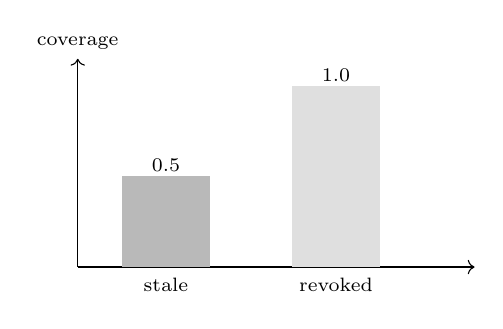
\begin{tikzpicture}[x=0.8cm,y=2.3cm]
  \draw[->] (0,0) -- (0,1.15) node[above, font=\scriptsize] {coverage};
  \draw[->] (0,0) -- (6.3,0);
  \fill[gray!55] (0.7,0) rectangle (2.1,0.5);
  \fill[gray!25] (3.4,0) rectangle (4.8,1.0);
  \node[font=\scriptsize] at (1.4,-0.10) {stale};
  \node[font=\scriptsize] at (4.1,-0.10) {revoked};
  \node[font=\scriptsize] at (1.4,0.56) {0.5};
  \node[font=\scriptsize] at (4.1,1.06) {1.0};
\end{tikzpicture}

\vspace{1mm}
{\scriptsize Historical projection over the same six raw observations: \textbf{3 states $\rightarrow$ 6 states $\rightarrow$ 3 states} (trusted $\rightarrow$ revoked $\rightarrow$ restored); raw digest unchanged.}
\caption{RQ3: stale trust hides controlled meaningful state; revocation restores coverage, while trust changes reinterpret preserved history without rewriting the raw archive.}
\label{fig:defeasible}
\end{figure}

\subsection{RQ4: Bounded Maintenance}
Phase~15 freezes four rules with priority scores 150, 84, 80, and 11 and budget two. The scheduler selects two rules and preserves unrelated lifecycle states. This demonstrates deterministic bounded selection, not an optimal scoring policy.

\subsection{RQ5: Operational Robustness}
The accepted Phase~19 combined study requests 15 runs over five targets. Nine succeed, six are externally unavailable, none is a StateScout run-error, and three targets are evaluable. A later replication remains 3/5 evaluable but changes TodoMVC stability.

Phase~20 produces a 256-state synthetic graph with 271 transitions/attempts and 16 injected failed probes. Interrupting at attempt 100 and resuming reaches the same final canonical graph as uninterrupted exploration; corrupted checkpoints are rejected. The depth-32 Playwright workflow produces 33 states, 32 transitions, and 496 replay-step observations; interrupting at 10 attempts and resuming to 32 also reaches the same final graph.

\section{Discussion}
\subsection{Abstraction as Cross-Run Trust}
The results support a distinction between classification and governance. APE establishes adaptive abstraction refinement/model rebuilding as prior art~\cite{gu2019ape}. StateScout's candidate novelty is therefore narrower: one run's identity is frozen, while later evidence changes explicit rule trust across runs.

\subsection{Observer Completeness}
The two v4 misses are observer-coverage failures. A targeted-content diagnostic fixes them, but globally fingerprinting arbitrary body text may create new false splits from feeds, timestamps, ads, or personalized content.

\subsection{Preserved History Is Not Retroactive Completeness}
Reprojection can reveal distinctions that were already recorded. It cannot reconstruct descendants or actions that an earlier false merge prevented from being explored.

\subsection{Temporal Variability and Replay Cost}
The public replication changes TodoMVC stability while W3C remains graph-unstable and Selenium remains stable. The depth-32 fixture requires 496 replay-step observations; wall-clock timings are too noisy for a complexity claim, but the structural count exposes replay cost.

\section{Threats to Validity}
Most controlled fixtures and labels were designed by the same researcher who implemented StateScout. Ground truth was repeatedly frozen before the corresponding change, negative results were retained, and Phase~21 freezes source, benchmarks, and tests during paper writing. These practices reduce but do not eliminate bias.

The production observer is operational rather than complete. The controlled corpus is small and diagnostic. The public study has five targets, with three evaluable in the accepted run. Behavior signatures are bounded evidence, not proof of semantic equivalence. The safe-only policy constrains the observable action space.

No confidence intervals are reported for public-site stability or performance. Phase~20 timing is single-machine observational data. Fingerprint generations were developed sequentially after earlier failures.

We do not reproduce Judge, FragGen, WebEmbed, or all modern baselines on this corpus and make no state-of-the-art classifier claim. APE also establishes dynamic abstraction refinement and model rebuilding as prior art~\cite{gu2019ape}. The remaining novelty claim is qualified as "to our knowledge, in the reviewed literature."

\section{Artifact and Reproducibility}
The frozen artifact exposes strict typecheck/tests, a deterministic controlled reproduction command, a separate public-site replication command, and SHA-256 provenance for quantitative paper assets. Protected Git-tree identities prevent paper editing from silently changing source, benchmarks, or tests.

For double-anonymous review, the artifact will be distributed through an anonymized repository/archive that does not expose author identity.

\section{Conclusion}
StateScout does not propose a universally optimal web-state classifier. It studies an explicit cross-run trust lifecycle around a learned abstraction assumption. The frozen experiments show that dynamic-looking syntax can be meaningful in context, stale trust can hide reachable state, later evidence can justify revocation, preserved history can retain recorded distinctions under changing trust, and interrupted exploration can resume to the same controlled graph.

The resulting design principle is narrow: web UI state equivalence can be represented as evidence-backed, revisable cross-run trust whose history survives the current abstraction.

\section*{Acknowledgment}
\textbf{Use of generative AI.} OpenAI ChatGPT was used during software development and manuscript preparation for interactive coding assistance, code and documentation review, literature-search assistance, language drafting/editing, and generation/refinement of reporting scripts and figure specifications. The author independently executed and reviewed the experiments, verified reported numerical results against the frozen research artifact, checked cited references and claim boundaries, and reviewed all AI-assisted text, code, and figures before inclusion.

\bibliographystyle{IEEEtran}
\bibliography{../references}
\end{document}
